\documentclass[10pt]{article}
\usepackage[OE]{express}
\usepackage{float}
\usepackage{booktabs}
\usepackage{menukeys}
\usepackage[normalem]{ulem}
\providecommand{\e}[1]{\ensuremath{\times 10^{#1}}} 
\providecommand{\mb}[1]{\mathbf{#1}}
\providecommand{\mh}[1]{\mathbf{\hat{#1}}}
\providecommand{\bs}[1]{\boldsymbol{#1}} 
\providecommand{\intinf}{\int_{-\infty}^{\infty}}

\begin{document}
\title{Single-fluorophore orientation determination with multiview polarized
  illumination: modeling and microscope design}

\author{Talon Chandler,\authormark{1,*} Shalin Mehta,\authormark{1,2,3} Hari
  Shroff,\authormark{4,5} Rudolf Oldenbourg,\authormark{2,6} and Patrick J. La
  Rivi\`ere\authormark{1,5}}
\address{\authormark{1}University of Chicago, Department of Radiology, Chicago, Illinois 60637, USA\\
  \authormark{2}Marine Biological Laboratory, Bell Center, Woods Hole, Massachusetts 02543, USA\\
  \authormark{3}(present address) Chan Zuckerberg Biohub, San Francisco, California 94158, USA\\
  \authormark{4}Section on High Resolution Optical Imaging, National Institute
  of Biomedical Imaging and Bioengineering, National Institutes of Health,
  Bethesda, Maryland 20892, USA\\
  \authormark{5}Marine Biological Laboratory, Whitman Center, Woods Hole,
  Massachusetts 02543, USA\\
  \authormark{6}Brown University, Department of Physics, Providence, Rhode
  Island 02912, USA}
\email{*talonchandler@talonchandler.com} %% email address is required

%%%%%%%%%%%%%%%%%%% abstract and OCIS codes %%%%%%%%%%%%%%%%
\begin{abstract}
  We investigate the use of polarized illumination in multiview microscopes for
  determining the orientation of single-molecule fluorescence transition
  dipoles. First, we relate the orientation of single dipoles to measurable
  intensities in multiview microscopes and develop an information-theoretic
  metric---the solid-angle uncertainty---to compare the ability of multiview
  microscopes to estimate the orientation of single dipoles. Next, we compare
  a broad class of microscopes using this metric---single- and dual-view
  microscopes with varying illumination polarization, illumination numerical
  aperture (NA), detection NA, obliquity, asymmetry, and exposure. We find that
  multi-view microscopes can measure all dipole orientations, while the
  orientations measurable with single-view microscopes is halved because of
  symmetries in the detection process. We also find that choosing a small
  illumination NA and a large detection NA are good design choices, that
  multiview microscopes can benefit from oblique illumination and detection, and
  that asymmetric NA microscopes can benefit from exposure asymmetry.
\end{abstract}

\ocis{(110.0110) Imaging systems; (180.2520) Fluorescence microscopy; (180.0180)
  Microscopy; (180.6900) Three-dimensional microscopy; (130.5440)
  Polarization-selective devices; (260.5430) Polarization.}

%%%%%%%%%%%%%%%%%%%%%%% References %%%%%%%%%%%%%%%%%%%%%%%%%
%% Comment before submission
% \bibliography{paper}
% \bibliographystyle{osajnl}


%% Copy .bbl and uncomment these before submission
% \begin{thebibliography}{99}
% \bibitem{gallo99} K. Gallo and G. Assanto, ``All-optical diode based on second-harmonic generation in an asymmetric waveguide,'' \josab {\bfseries 16}(2), 267--269 (1999).
% \end{thebibliography}


\begin{thebibliography}{10}
\newcommand{\enquote}[1]{``#1''}

\bibitem{peterman2001}
E.~J. Peterman, H.~Sosa, L.~S. Goldstein, and W.~E. Moerner, \enquote{Polarized
  fluorescence microscopy of individual and many kinesin motors bound to
  axonemal microtubules,} Biophys. J. \textbf{81}, 2851--2863 (2001).

\bibitem{forkey2003}
J.~N. Forkey, M.~E. Quinlan, M.~A. Shaw, J.~E.~T. Corrie, and Y.~E. Goldman,
  \enquote{Three-dimensional structural dynamics of myosin {V} by
  single-molecule fluorescence polarization,} \nat \textbf{422}, 399--404
  (2003).

\bibitem{backer2016}
A.~S. Backer, M.~Lee, and W.~E. Moerner, \enquote{Enhanced {DNA} imaging using
  super-resolution microscopy and simultaneous single-molecule orientation
  measurements,} in \enquote{Conference on Lasers and Electro-Optics,}
  (Optical Society of America, 2016), p. JTh4B.4.

\bibitem{mehta2016}
S.~B. Mehta, M.~McQuilken, P.~J. La~Rivi\`ere, P.~Occhipinti, A.~Verma,
  R.~Oldenbourg, A.~S. Gladfelter, and T.~Tani, \enquote{Dissection of
  molecular assembly dynamics by tracking orientation and position of single
  molecules in live cells,} Proc. Natl. Acad. Sci. U.S.A. \textbf{113},
  E6352--E6361 (2016).

\bibitem{demay2011}
B.~DeMay, N.~Noda, A.~Gladfelter, and R.~Oldenbourg, \enquote{Rapid and
  quantitative imaging of excitation polarized fluorescence reveals ordered
  septin dynamics in live yeast,} Biophys. J. \textbf{101}, 985--994 (2011).

\bibitem{mcquilken2017}
M.~McQuilken, M.~S. Jentzsch, A.~Verma, S.~B. Mehta, R.~Oldenbourg, and A.~S.
  Gladfelter, \enquote{Analysis of septin reorganization at cytokinesis using
  polarized fluorescence microscopy,} Front. Cell Dev. Biol. \textbf{5}, 42
  (2017).

\bibitem{anantharam2010}
A.~Anantharam, B.~Onoa, R.~H. Edwards, R.~W. Holz, and D.~Axelrod,
  \enquote{Localized topological changes of the plasma membrane upon exocytosis
  visualized by polarized {TIRFM},} J. Cell Biol. \textbf{188}, 415--428
  (2010).

\bibitem{backlund2014}
M.~P. Backlund, M.~D. Lew, A.~S. Backer, S.~J. Sahl, and W.~E. Moerner,
  \enquote{The role of molecular dipole orientation in single-molecule
  fluorescence microscopy and implications for super-resolution imaging,}
  ChemPhysChem \textbf{15}, 587--599 (2014).

\bibitem{lieb2004}
M.~A. Lieb, J.~M. Zavislan, and L.~Novotny, \enquote{Single-molecule
  orientations determined by direct emission pattern imaging,} J. Opt. Soc. Am.
  B \textbf{21}, 1210--1215 (2004).

\bibitem{backer2014}
A.~S. Backer and W.~E. Moerner, \enquote{Extending single-molecule microscopy
  using optical {F}ourier processing,} J. Phys. Chem. B \textbf{118},
  8313--8329 (2014).

\bibitem{agrawal2012}
A.~Agrawal, S.~Quirin, G.~Grover, and R.~Piestun, \enquote{Limits of 3{D}
  dipole localization and orientation estimation for single-molecule imaging:
  towards {G}reen's tensor engineering,} Opt. Express \textbf{20}, 26667--26680
  (2012).

\bibitem{toprak2006}
E.~Toprak, J.~Enderlein, S.~Syed, S.~A. McKinney, R.~G. Petschek, T.~Ha, Y.~E.
  Goldman, and P.~R. Selvin, \enquote{Defocused orientation and position
  imaging ({DOPI}) of myosin {V},} Proc. Natl. Acad. Sci. U.S.A. \textbf{103}, 6495--6499 (2006).

\bibitem{debarre2004}
A.~D{\'e}barre, R.~Jaffiol, C.~Julien, D.~Nutarelli, A.~Richard,
  P.~Tch{\'e}nio, F.~Chaput, and J.-P. Boilot, \enquote{Quantitative
  determination of the 3{D} dipole orientation of single molecules,} Eur. Phys.
  J. D. \textbf{28}, 67--77 (2004).

\bibitem{shribak2003}
M.~Shribak and R.~Oldenbourg, \enquote{Techniques for fast and sensitive
  measurements of two-dimensional birefringence distributions,} Appl. Opt.
  \textbf{42}, 3009--3017 (2003).

\bibitem{fourkas2001}
J.~T. Fourkas, \enquote{Rapid determination of the three-dimensional
  orientation of single molecules,} Opt. Lett. \textbf{26}, 211--213 (2001).

\bibitem{tyo2006}
J.~S. Tyo, D.~L. Goldstein, D.~B. Chenault, and J.~A. Shaw, \enquote{Review of
  passive imaging polarimetry for remote sensing applications,} Appl. Opt.
  \textbf{45}, 5453--5469 (2006).

\bibitem{lu2008}
C.-Y. Lu and D.~A.~Vanden Bout, \enquote{Analysis of orientational dynamics of
  single fluorophore trajectories from three-angle polarization experiments,}
  J. Chem. Phys. \textbf{128}, 244501 (2008).

\bibitem{wu2013}
Y.~Wu, P.~Wawrzusin, J.~Senseney, R.~S. Fischer, R.~Christensen, A.~Santella,
  A.~G. York, P.~W. Winter, C.~M. Waterman, Z.~Bao, D.~A. Colon-Ramos,
  M.~McAuliffe, and H.~Shroff, \enquote{Spatially isotropic four-dimensional
  imaging with dual-view plane illumination microscopy,} Nat. Biotechnol.
  \textbf{31}, 1032--1038 (2013).

\bibitem{keller2015}
R.~K. Chhetri, F.~Amat, Y.~Wan, B.~Hockendorf, W.~C. Lemon, and P.~J. Keller,
  \enquote{Whole-animal functional and developmental imaging with isotropic
  spatial resolution,} Nat. Methods \textbf{12}, 1171--1178 (2015).

\bibitem{wu2016}
Y.~Wu, P.~Chandris, P.~W. Winter, E.~Y. Kim, V.~Jaumouill{\'e}, A.~Kumar,
  M.~Guo, J.~M. Leung, C.~Smith, I.~Rey-Suarez, H.~Liu, C.~M. Waterman, K.~S.
  Ramamurthi, P.~J. La~Rivi\`ere, and H.~Shroff, \enquote{Simultaneous
  multiview capture and fusion improves spatial resolution in wide-field and
  light-sheet microscopy,} Optica \textbf{3}, 897--910 (2016).

\bibitem{wu2017}
Y.~Wu, A.~Kumar, C.~Smith, E.~Ardiel, P.~Chandris, R.~Christensen,
  I.~Rey-Suarez, M.~Guo, H.~Vishwasrao, J.~Chen, J.~Tang, A.~Upadhyaya,
  P.~La~Rivi\`ere, and H.~Shroff, \enquote{Reflective imaging improves
  resolution, speed, and collection efficiency in light sheet microscopy,}
  bioRxiv  (2017).

\bibitem{kay1993}
S.~M. Kay, \emph{Fundamentals of statistical signal processing} (Prentice Hall
  PTR, 1993).

\bibitem{anderson1958}
  T.~W. Anderson, \emph{An introduction to multivariate statistical analysis}
(Wiley, 1958).

\bibitem{coe2009}
D.~Coe, \enquote{Fisher matrices and confidence ellipses: a quick-start guide
  and software,} arXiv preprint arXiv:0906.4123  (2009).

\bibitem{walt2011}
S.~van~der Walt, S.~C. Colbert, and G.~Varoquaux, \enquote{The {N}um{P}y array:
  a structure for efficient numerical computation,} CoRR \textbf{abs/1102.1523}
  (2011).

\bibitem{meurer2017}
A.~Meurer, C.~P. Smith, M.~Paprocki, O.~\v{C}ert\'{i}k, S.~B. Kirpichev,
  M.~Rocklin, A.~Kumar, S.~Ivanov, J.~K. Moore, S.~Singh, T.~Rathnayake,
  S.~Vig, B.~E. Granger, R.~P. Muller, F.~Bonazzi, H.~Gupta, S.~Vats,
  F.~Johansson, F.~Pedregosa, M.~J. Curry, A.~R. Terrel, v.~Rou\v{c}ka,
  A.~Saboo, I.~Fernando, S.~Kulal, R.~Cimrman, and A.~Scopatz,
  \enquote{Sym{P}y: symbolic computing in {P}ython,} PeerJ Computer Science
  \textbf{3}, e103 (2017).

\bibitem{hunter2007}
J.~D. Hunter, \enquote{Matplotlib: A {2D} graphics environment,} Computing In
  Science \& Engineering \textbf{9}, 90--95 (2007).

\bibitem{vispy}
L.~Campagnola, A.~Klein, E.~Larson, A.~Griffiths, C.~Rossant, N.~P. Rougier,
  I.~Zaid, M.~S. Suraj, A.~Taylor, sylm21, M.~F. Kaptan, A.~J. Champandard,
  karlcz, nippoo, Siddharth, X.~Gao, C.~GESTES, bdurin, J.~D. Reaver,
  R.~McMullen, FiachAntaw, T.~Mansencal, M.~Dartiailh, StephenWest, J.~Kieffer,
  G.~Baty, R.~Peters, macduff111, E.~S. de~Andrade, and D.~Rufat,
  \enquote{vispy: Version 0.4.0,}  (2015).

\bibitem{bowman2008}
J.~C. Bowman and A.~Hammerlindl, \enquote{Asymptote: A vector graphics
  language,} TUGBOAT \textbf{29}, 288--294 (2008).

\bibitem{nov2006}
L.~Novotny and B.~Hecht, \emph{Principles of Nano-Optics} (Cambridge University, 2006).

\bibitem{levoy2006}
M.~Levoy, R.~Ng, A.~Adams, M.~Footer, and M.~Horowitz, \enquote{Light field
  microscopy,} in \enquote{ACM SIGGRAPH 2006 Papers,}  (ACM, New York, NY, USA,
  2006), SIGGRAPH '06, pp. 924--934.

\end{thebibliography}


\section{Introduction}\label{sec:intro}
The orientation of single-molecule fluorescence transition dipoles is a valuable
reporter for biological processes. By imaging biological samples with
fluorescent probes that are fixed to known structures, researchers have studied
the dynamics of motor proteins \cite{peterman2001, forkey2003}, DNA
\cite{backer2016}, actin \cite{mehta2016}, septin \cite{demay2011,
  mcquilken2017}, and membranes \cite{anantharam2010}. The number of techniques
available to biologists for measuring the orientation of single dipoles in live
cells is continually expanding. A recent review \cite{backlund2014} identified
three major categories of single-dipole orientation determination techniques:

\textbf{Spatial/angular variation of emission} techniques image single molecules
and use the distribution of intensity in the back focal plane \cite{lieb2004} or
in the image plane \cite{backer2014} to estimate their dipole
orientation. Information-theoretically optimal techniques in this category use
defocusing or phase masks in the back focal plane to encode orientation and
position information in the image \cite{agrawal2012}. These techniques can
estimate the orientation of dipoles in all orientations and only require a
single frame of intensity measurements, but they require complex reconstruction
algorithms, expensive high numerical aperture (NA) optics, and sensitive
detectors. Furthermore, these techniques spread the signal from a single
molecule over a large area on the detector, so they suffer from a poor
signal-to-noise ratio \cite{toprak2006}.

\textbf{Spatial variation of illumination polarization} techniques vary the
polarization and intensity in the illumination path to excite dipoles in
specific orientations in the focal volume \cite{debarre2004}. Although these
techniques can accurately estimate the orientation of dipoles in all
orientations, they require scanning which makes acquisition time a concern in
live-cell imaging.

\textbf{Polarized illumination or detection} techniques vary the polarization of
light in the illumination or detection paths and exploit the anisotropic
absorption and emission patterns of single molecules to estimate their dipole
orientation. By illuminating and detecting from the focal plane, not just the
focal point, these techniques can estimate the orientation of many dipoles in
parallel without scanning. These techniques are easy to implement---changing the
illumination or detection polarization is simple with a polarization splitter
\cite{mehta2016} or universal compensator/polarizer \cite{shribak2003}---and the
reconstruction methods are straightforward \cite{fourkas2001, mehta2016,
  backer2016}. Also, these techniques keep the signal from a single molecule
localized on the detector, so they have a signal-to-noise ratio advantage over
defocusing and phase masking techniques. The main drawback is that these
techniques require several intensity measurements under different polarization
orientations to estimate the orientation of a single dipole. Despite the
requirement for multiple measurements, polarized illumination or detection
methods are good choices for live-cell imaging because of their combination of
speed and ease of implementation.

To develop a polarized illumination or detection technique we need to choose a
method for varying the polarization and place it in the illumination or
detection path. The simplest and most inexpensive way to vary the polarization
is with a division-of-time (DoT) polarizer using a rotating polarizer or a
universal compensator/polarizer. Other polarization methods
(division-of-amplitude, division-of-focal-plane) are more expensive and require
additional alignment or interpolation \cite{tyo2006}. The simplicity of DoT
polarization comes at the expense of temporal resolution---intensity
measurements are made one after the other which increases the acquisition
time. If we place the DoT polarizer in the detection path, we will block
valuable photons from reaching the detector which leads to unnecessary exposure
to the sample \cite{demay2011}. By placing the DoT polarizer in the illumination
arm we minimize exposure to the sample. We focus on DoT polarized illumination
in this paper because of its combination of simplicity and low sample exposure.

All single-dipole orientation determination methods suffer from some degree of
anisotropic orientation uncertainty, i.e., some dipole orientations cannot be
determined as precisely as others. In some cases the orientation cannot be
determined at all---the forward model can be degenerate for specific dipole
orientations \cite{fourkas2001, lu2008}. We feel that the importance of
isotropic orientation uncertainty has been underappreciated. To our knowledge,
the only authors who have considered anisotropic orientation uncertainty in 3D
have only analyzed a subset of dipole orientations \cite{agrawal2012}. Our view
is that an ideal technique for determining the orientation of single dipoles can
reconstruct the orientation with a small and nearly uniform uncertainty for all
dipole orientations.

Recently, there has been increasing interest in multiview microscopy techniques
for biological imaging \cite{wu2013, keller2015, wu2016, wu2017}. Multiview
microscopes offer two major advantages over single-view microscopes. First,
multiview microscopes can achieve nearly isotropic resolution compared to the
anisotropic resolution of single-view microscopes whose axial resolution is
reduced by at least a factor of two compared to lateral resolution. Second,
multiview microscopes can use light-sheet illumination to reduce phototoxicity
while reusing parts of the optical path for both illumination and detection. For
example, if two orthogonal objectives are focused on the same point, then the
objectives can alternate roles as the light-sheet illumination path and as the
detection path. Light-sheet illumination offers a major reduction of
phototoxicity because a light sheet only illuminates in-focus regions while
other widefield and confocal approaches inevitably illuminate out-of-focus
regions. Together, these advantages make multiview microscopes good candidates
for imaging live biological specimens for long periods.

In this work we explore the use of polarized illumination in multiview
microscopes for determining the orientation of single dipoles. Existing
multiview microscopes can easily be outfitted with fast-switching polarizers
that do not degrade image quality, so polarized illumination is a natural way to
augment multiview microscopes for measuring the orientation of single
dipoles. Furthermore, multiview microscopes can achieve nearly isotropic
resolution while delivering selective illumination. We find that multiview
microscopes also provide a small and uniform orientation uncertainty for single
dipoles in all orientations. We also find that single-view microscopes have
symmetries that can be broken by adding a second view. This reduction of
degeneracy allows multiview microscopes to uniquely determine the orientation of
single dipoles.

In section \ref{methods} we develop the theory required to model polarized
illumination microscopes, and we develop metrics to compare microscope
designs. In section \ref{results} we compare the results for a wide range of
multiview microscope designs. Finally, in section \ref{discussion} we discuss
the results and their impact on polarized multiview microscope design.

\section{Methods}\label{methods}
In this section we develop a method to compare multiview polarized illumination
microscopes for the task of reconstructing dipole orientations. In sections
\ref{excitation}--\ref{forward} we develop a model for the intensity collected
with a fixed illumination and detection configuration as a function of the
dipole orientation. In section \ref{designs} we list a variety of ways to
combine these intensity measurements into experimentally realizable polarized
illumination microscopes. Finally, in section \ref{metrics} we develop metrics
that we will use to compare these microscopes.

We use roman type for scalars, e.g., $\phi$, $\theta$; bold lowercase type for
vectors, e.g., $\mb{r}, \bs{\mu}$; hats for unit vectors, e.g.,
$\mh{r}, \hat{\bs{\mu}}$; and bold capital type for matrices, e.g.,
$\mb{R}, \mb{F}$.

\subsection{Absorption efficiency}\label{excitation}
In this section we will calculate the \emph{absorption efficiency} of a single
dipole---the fraction of the incident power that is absorbed by the
dipole. Our approach is inspired by Fourkas \cite{fourkas2001}, but here we
calculate the absorption efficiency instead of the detection efficiency.

\begin{figure}[H]
\centering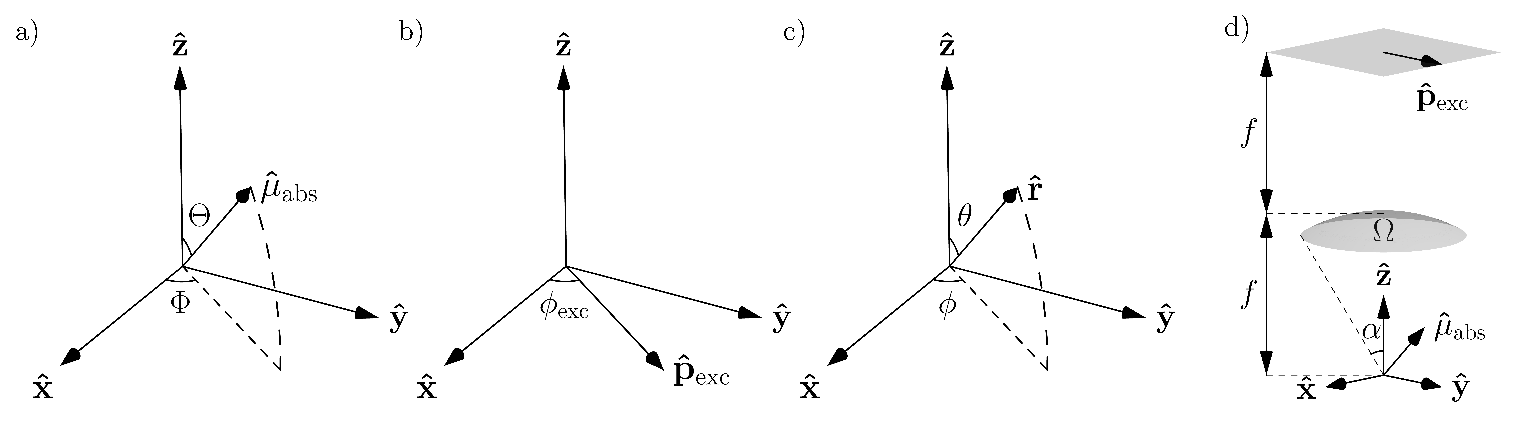
\includegraphics[width=\textwidth]{frames}
\caption{Coordinate systems for a) the absorption dipole moment
  $\hat{\bs{\mu}}_{\text{abs}}$, b) the polarizer transmission axis
   $\hat{\mb{p}}_{\text{exc}}$, and c) the dummy integration vector
  $\hat{\mb{r}}$. d) The scene consists of a single molecule at the focal point
  of an objective lens with a polarizer in the aperture plane.}
\hypertarget{typo}{}
\label{fig:coordinates}
\end{figure}

We consider a single molecule with a fixed absorption dipole moment
$\hat{\bs{\mu}}_{\text{abs}}$ that we express in spherical coordinates $\Theta$
and $\Phi$ [see Fig. \ref{fig:coordinates}(a)] as
\begin{align}
  \hat{\bs{\mu}}_{\text{abs}}(\Theta, \Phi) = \sin\Theta\cos\Phi\hat{\mb{x}} + \sin\Theta\sin\Phi\hat{\mb{y}} + \cos\Theta\hat{\mb{z}} \label{eq:mu}.
\end{align}
We place the molecule in the focal plane of an ideal, aplanatic,
polarization-preserving objective lens with its optical axis aligned with the
$\mh{z}$ axis. Next, we place a polarizer in the aperture plane with a variable
transmission axis $\hat{\mb{p}}_{\text{exc}}$ that we express as
\begin{align}
 \hat{\mb{p}}_{\text{exc}}(\phi_{\text{exc}}) = \cos\phi_{\text{exc}}\hat{\mb{x}} +
\sin\phi_{\text{exc}}\hat{\mb{y}},\label{eq:excfield}
\end{align}
where $\phi_{\text{exc}}$ is the angle between the transmission axis of the
polarizer and the positive $\mh{x}$ axis [see Fig.
\ref{fig:coordinates}(b)]. Finally, we place a spatially incoherent and
spatially uniform light source (or its image) in the aperture plane to
illuminate the focal plane. In this geometry each point in the sample is
illuminated by a range of angles that can be changed by adjusting the radius of
the diaphragm in the aperture plane. We denote the set of illuminated angles by
$\Omega$ [see Fig. \ref{fig:coordinates}(d)]. If we use unit vectors
$\hat{\mb{r}}$ expressed in spherical coordinates $\theta$ and $\phi$ [see
Fig. \ref{fig:coordinates}{(c)] as
  \begin{align}
   \hat{\mb{r}}(\theta, \phi) = \sin\theta\cos\phi\hat{\mb{x}} + \sin\theta\sin\phi\hat{\mb{y}} + \cos\theta\hat{\mb{z}}, 
  \end{align}
  then the set of angles $\Omega$ can be expressed as
  \begin{align}
  \Omega = \{\phi, \theta\ |\ 0 < \phi \leq 2\pi, 0 < \theta \leq \alpha\},
  \end{align}
  where $\alpha$ is the angle between the optical axis and the most oblique
  illuminating ray. Equivalently, $\alpha$ can be expressed in terms of NA using
  \begin{align}
    \text{NA} = n\sin\alpha, 
  \end{align}
  where $n$ is the index of refraction of the sample medium. Note that the NA of
  the objective is always greater than or equal to the illumination NA because
  we can underfill the aperture plane.
  
  The objective focuses the light by applying a position-dependent rotation to
  the electric field which we model by multiplying the incident electric field
  $\hat{\mb{p}}_{\text{exc}}$ by a position-dependent rotation matrix
  \begin{align}
  \mb{R}(\mh{r}) &= \begin{bmatrix} \cos\theta\cos^2\phi + \sin^2\phi & (\cos\theta -1)\sin\phi\cos\phi & \sin\theta\cos\phi\\ (\cos\theta - 1)\sin\phi\cos\phi & \cos\theta\sin^2\phi + \cos^2\phi & \sin\theta\sin\phi \\ -\sin\theta\cos\phi& -\sin\theta\sin\phi & \cos\theta \end{bmatrix} \label{eq:rot_mat}.
  \end{align}
  Note the difference of signs between Eq.
  (\ref{eq:rot_mat}) and the rotation matrix given by
    Fourkas---our matrix rotates rays propagating towards the sample while
    Fourkas' matrix rotates rays propagating away from the sample.

  To find the absorption efficiency $\eta_{\text{abs}}$ of a single dipole if
  it were illuminated by a single ray, we take the unit incident electric field
  $\hat{\mb{p}}_{\text{exc}}$, take the dot product with the absorption dipole
  moment, then take the modulus squared
    \begin{align}
      \eta_{\text{abs}}^{\text{ray}} &= |\hat{\bs{\mu}}_{\text{abs}}\cdot\mh{p}_{\text{exc}}|^2. \label{eq:singleray}
    \end{align}

    To find the absorption efficiency of a single dipole, we integrate over
    all illumination rays and divide by the total incident power which gives the
    vector expression
\begin{align}
  \eta_{\text{abs}} = \frac{\int_{\Omega}d\mh{r}|\hat{\bs{\mu}}_{\text{abs}}\cdot\mb{R}(\mh{r})\mh{p}_{\text{exc}}|^2}{\int_{\Omega}d\mh{r}}\label{eq:abs}. 
\end{align}

We substitute Eqs. (\ref{eq:mu})--(\ref{eq:rot_mat}) into
Eq. (\ref{eq:abs}), evaluate the integrals, and simplify to
express the absorption efficiency in scalar notation as
\begin{align}
  \eta_{\text{abs}} &= D\{A + B\sin^{2}{\Theta} + C\sin^{2}{\Theta} \cos{[2 (\Phi - \phi_{\text{exc}}})]\}\label{eq:scalarabs}
\end{align}
where
\begin{subequations}
\begin{align}
  A &= \frac{1}{4} - \frac{3}{8} \cos{\alpha } + \frac{1}{8} \cos^{3}{\alpha }\\
  B &= \frac{3}{16} \cos{\alpha } - \frac{3}{16} \cos^{3}{\alpha }\\
  C &= \frac{7}{32} - \frac{3}{32} \cos{\alpha } - \frac{3}{32} \cos^{2}{\alpha } - \frac{1}{32} \cos^{3}{\alpha}\\
  D &= \frac{4}{3(1 - \cos\alpha)}.
\end{align}\label{eq:coefficients}%
\end{subequations}
Note that the factor $D$ keeps the specimen irradiance constant for any value of
$\alpha$. We have kept $D$ as a multiplicative factor in
Eq. (\ref{eq:scalarabs}) to facilitate comparison with Fourkas' results, but
Eq. (\ref{eq:scalarabs}) can be simplified further by distributing $D$.

We can extend these results to light-sheet illumination created by scanning a
laser. If we shine a narrow, collimated, laser beam onto a galvanometer in the
aperture plane and scan the galvanometer, we create a weakly focused light sheet
in the sample. If we scan the beam in the sample with a velocity much less than
the beam waist radius divided by the coherence time, then the coherence of the
laser is rendered ineffectual by the scanning---the light sheet is effectively
composed of many incoherent beams. If we also ensure that the laser beam is
weakly focused, we can ignore the excitation caused by the small fields aligned
with the optical axis. Under slowly-scanned and weakly-focused light-sheet
illumination, dipoles in the sample will be excited as if a single plane wave
was incident. Therefore, we can find the absorption efficiency of a dipole in
this case by taking the limit of Eq. (\ref{eq:scalarabs}) as
$\alpha \rightarrow 0$ [or by plugging Eqs. (\ref{eq:mu}) and
(\ref{eq:excfield}) into Eq. (\ref{eq:singleray})] giving
\begin{align}
  \eta_{\text{abs}}^{\text{ray}} &= \sin^2\Theta\cos^2(\Phi - \phi_{\text{exc}}),
\end{align}
which is recognizable as Malus' law generalized to three dimensions. This means
that light-sheet illumination is approximately equivalent to low-NA illumination
with respect to the dipole orientations they excite. Notice that the
absorption efficiency can take its maximum range of values
($\eta_{\text{abs}} \in [0, 1]$) when $\alpha=0$.

\subsection{Detection efficiency}\label{detection}
In this section we will calculate the \emph{detection efficiency}---the fraction
of the power emitted by a single dipole that we detect. Fourkas calculated the
detection efficiency when an ideal objective with its optical axis aligned with
the $\mh{z}$ axis is focused on a single dipole and a polarizer is placed in
the aperture plane \cite{fourkas2001}. He found that
\begin{align}
  \eta_{\text{det}}^{\text{pol}} = A + B\sin^2\Theta + C\sin^{2}{\Theta} \cos{[2 (\Phi - \phi_{\text{det}}})], \label{eq:det_pol}
\end{align}
where $\phi_{\text{det}}$ is the angle between the transmission axis of the
detection polarizer and the positive $\mh{x}$ axis. 

To calculate the detection efficiency without a polarizer, we use Eq.
(\ref{eq:det_pol}) and take the sum of polarized detection efficiencies with
orthogonal polarizer orientations to find
\begin{align}
  \eta_{\text{det}} = 2(A + B\sin^2\Theta). \label{eq:scalardet}
\end{align}
In this case the detection efficiency only depends on $\Theta$, not $\Phi$,
because there is no detection polarizer. We have assumed that the absorption
dipole moment is equal to the emission dipole moment.

Note that $A$, $B$, and $C$ in Eq. (\ref{eq:coefficients}) are a factor of
$\frac{3}{2}$ larger than the expressions given by Fourkas. We found that
Fourkas' expressions were incorrectly normalized (the limit of
$\eta_{\text{det}}$ as $\alpha\rightarrow \frac{\pi}{2}$ should be
$\frac{1}{2}$), and the extra factor of $\frac{3}{2}$ corrects the error. The
extra factor of $\frac{3}{2}$ is a constant multiplicative factor, so the
correction is not angle-dependent which means that it does not affect Fourkas'
orientation reconstruction. However, the correction does mean that Fourkas'
algorithm underpredicts the total emitted intensity by a factor of
$\frac{3}{2}$.

Also note that the detection efficiency can take its maximum range of values
when $B$ takes its maximum value, i.e. when
$\alpha=\arccos\left(\frac{1}{\sqrt{3}}\right) \approx 54.7^{\circ}$. This means
that the maximum modulation of detected intensities will occur when we choose a
detection objective with $\alpha \approx 54.7^{\circ}$.

\subsection{Oblique illumination and detection}\label{oblique}
In sections \ref{excitation} and \ref{detection} we assumed that both the
illumination and detection objectives had $\mh{z}$ aligned optical axes, i.e.,
we assumed traditional epi- or transmitted light illumination. To extend the
forward model to oblique optical axes which allows for non-coincident
illumination and detection objectives, we express the dipole orientation in a
rotated coordinate frame using the following expressions
\begin{align}
    \Theta' &= \arccos\left(\sin\psi\cos\Phi\sin\Theta + \cos\psi\cos\Theta\right)\label{eq:thetap}\\
  \Phi' &=
          \begin{cases}
            \arccos\left(\dfrac{\cos\psi\cos\Phi\sin\Theta - \sin\psi\cos\Theta}{\sqrt{1 - (\sin\psi\cos\Phi\sin\Theta + \cos\psi\cos\Theta)^2}}\right) \ \ \ &0 \leq \Phi < \pi  \\
            -\arccos\left(\dfrac{\cos\psi\cos\Phi\sin\Theta - \sin\psi\cos\Theta}{\sqrt{1 - (\sin\psi\cos\Phi\sin\Theta + \cos\psi\cos\Theta)^2}}\right) \ \ \ &-\pi \leq \Phi < 0\\
          \end{cases}\label{eq:phip}
\end{align}
where $\psi$ is the angle of a right handed rotation about the $\mh{y}$ axis
that maps the $\mh{z}$ axis onto the new optical axis.

\subsection{Intensity measurements}\label{forward}
The detected intensity is proportional to the product of the sample irradiance
$I_{\text{in}}$, the absorption efficiency, and the detection efficiency
\begin{align}
  I \propto I_{\text{in}}\eta_{\text{abs}}\eta_{\text{det}}\label{eq:forward_frame},
\end{align}
where the proportionality depends on the exposure time, the molecular quantum
efficiencies, and other constant factors. Equation (\ref{eq:forward_frame}) is the
forward model for a single intensity measurement. Figure \ref{fig:single-frame}
shows the efficiencies in three representative geometries. Note that in all
cases there are multiple orientations that give the same intensity
measurement. This means that a single intensity measurement does not give us
enough information to reconstruct the orientation of a single dipole. Next, we
will consider combining several intensity measurements to create polarized
illumination microscopes that can reconstruct the orientation of single
dipoles.

\begin{figure}[H]
\centering\includegraphics[width=\textwidth]{single-frame}
\caption{Representative examples of single intensity measurements. Black dots
  indicate where the Cartesian unit vectors intersect the unit sphere. \newline
  \newline \textbf{Columns left to right:} 1) schematics where the solid line
  encloses the illumination solid angle, the dashed line encloses the detection
  solid angle, and the arrow indicates the transmission axis of the illumination
  polarizer; 2) the absorption efficiency, see Eq.  (\ref{eq:scalarabs}); 3) the
  detection efficiency, see Eq.  (\ref{eq:scalardet}); 4) the total efficiency,
  the product of the absorption and detection efficiencies.\newline \newline
  \textbf{Rows top to bottom:} 1) coincident illumination ($\text{NA} = 1.1$
  with $x$-polarized light) and detection (NA = 1.1); 2) non-coincident
  orthogonal illumination ($\text{NA} = 0.8$) and detection ($\text{NA} = 0.8$);
  3) non-coincident 135${}^{\circ}$-separated illumination ($\text{NA} = 0.8$)
  and detection ($\text{NA} = 0.8$). All simulations use $n=1.33$.}
  \label{fig:single-frame}
\end{figure}

\subsection{Polarized illumination microscope configurations}\label{designs}
One way to collect multiple intensity measurements is to add a universal
compensator/polarizer to the illumination arm and rapidly select the incident
polarization by changing $\phi_{\text{exc}}$ \cite{shribak2003}. All of the
microscopes we will consider in this paper use four polarizations per
illumination path with the polarization orientations separated by
45${}^{\circ}$.

We also consider several dual-view designs. We evaluate dual-view designs that
allow for illumination and detection from both objectives (see \cite{wu2013} for
a dual-view design). In all cases we consider the effect of varying the
illumination and detection numerical aperture. We also consider asymmetric NA
designs (see \cite{wu2017} for an asymmetric NA design) and the effect of
asymmetric sample exposures. Note that we use the word \emph{symmetry} to refer
to dual-view designs with identical objectives and sample exposures and the word
\emph{asymmetry} to refer to dual-view designs with objectives that have a
different NA or sample exposure.

All multiview microscopes are subject to steric constraints---the objectives
must not collide with the cover slip or each other. We only consider microscope
designs that meet these criteria.

\subsection{Evaluation metrics}\label{metrics}
Our goal is to evaluate the ability of a microscope design to estimate the
orientation of a single dipole (via parameters $\Theta$ and $\Phi$) from
intensity data. A common way to evaluate the ability to estimate the parameters
$\Theta$ and $\Phi$ from the data is to calculate the Cram\'er-Rao lower bound
(CRLB) for each parameter \cite{kay1993}. The CRLBs are given by the diagonal
elements of the inverse of the Fisher information matrix, and they give the
minimum variance of an unbiased estimator for each parameter. For each
microscope design and dipole orientation we calculate the Fisher information
matrix. We assume that the detected intensities are Poisson distributed, so the
Fisher information matrix is given by
\begin{align}
  \mb{F} &= \sum_{k=1}^N \frac{1}{I_k}
  \begin{bmatrix}
    \dfrac{\partial I_k}{\partial \Theta}\dfrac{\partial I_k}{\partial \Theta}&\dfrac{\partial I_k}{\partial \Theta}\dfrac{\partial I_k}{\partial \Phi}\\\\
    \dfrac{\partial I_k}{\partial \Theta}\dfrac{\partial I_k}{\partial \Phi}&\dfrac{\partial I_k}{\partial \Phi}\dfrac{\partial I_k}{\partial \Phi}\\    
  \end{bmatrix}
\end{align}
where $I_k$ is the $k$th intensity measurement in a microscope that uses $N$
intensity measurements. Agrawal et. al. used the square root of the product of
the CRLBs multiplied by the Jacobian determinant,
$\sin\Theta\sqrt{\mb{F}^{-1}_{0,0}\mb{F}^{-1}_{1,1}}$, to find the area of
uncertainty in parameter space \cite{agrawal2012}.

CRLBs and the associated area of uncertainty are parameterization dependent,
i.e., if we choose a different coordinate system these metrics will change. We
would like to compare microscope designs without choosing a parameterization, so
instead we use
\begin{align}
  \sigma_{\Omega} &\equiv \sin\Theta\sqrt{\text{det}\{\mb{F}^{-1}\}}
\end{align}
as our evaluation metric. We calculate the determinant of the inverse Fisher
information matrix---a parameterization-independent value called the
\emph{generalized variance} \cite{anderson1958}---take the square root, then
multiply by the Jacobian determinant, $\sin\Theta$. We call $\sigma_{\Omega}$
the \emph{solid-angle uncertainty} because it has units of steradians and is a
parameterization independent measure of the orientation uncertainty.

For each microscope we calculate $\sigma_{\Omega}$ at 10,000 approximately
equally spaced points on the unit sphere. A desirable microscope design will
have a small solid-angle uncertainty that is uniform for all dipole
orientations. The most straightforward way to find the location and scale of the
solid-angle uncertainty is to use the mean and variance, respectively. However,
the solid-angle uncertainty can take extremely large values, e.g., when a
fluorescent dipole is aligned with the optical axis of a single excitation
objective. Such large values can change the mean and variance dramatically
depending on the sample points, so we use the median and median absolute
deviation (MAD)---the median of the data's absolute difference from the
median---as robust alternatives to the mean and variance.

To compare microscopes with different numbers of intensity measurements fairly,
we kept the irradiance incident on the sample constant by choosing
$I_{\text{in}} = \frac{4000}{N}$. Note that $I_{\text{in}}$ is a measure of
irradiance to the sample, not the detected intensity or the total intensity
emitted by the molecule.

We also use the Fisher information matrix to calculate uncertainty ellipses for
each microscope and dipole orientation. The general equation of an ellipse
with axis radii $a$ and $b$ and rotation angle $\gamma$ is
\begin{align}
  \frac{(x\cos\gamma + y\sin\gamma)^2}{a^2} + \frac{(x\sin\gamma - y\cos\gamma)^2}{b^2} =1. 
\end{align}%
We calculate the ellipse parameters in terms of the Fisher information matrix
using the following set of equations
\begin{align}
  \sigma_x &= \sqrt{\mb{F}^{-1}_{0,0}} \label{eq:first}\\
  \sigma_y &= \sin\Theta\sqrt{\mb{F}^{-1}_{1,1}} \label{eq:second}\\ 
  \sigma_{xy} &= \sin\Theta\sqrt{\mb{F}^{-1}_{1,0}} \label{eq:third}\\  
  a^2 &= \frac{\sigma_x^2 + \sigma_y^2}{2} + \sqrt{\frac{(\sigma_x^2 - \sigma_y^2)^2}{4} + \sigma_{xy}^2}\\
  b^2 &= \frac{\sigma_x^2 + \sigma_y^2}{2} - \sqrt{\frac{(\sigma_x^2 - \sigma_y^2)^2}{4} + \sigma_{xy}^2}\\
  \gamma &= \frac{1}{2}\text{arctan}\left(\frac{2\sigma_{xy}}{\sigma_x^2 - \sigma_y^2}\right). \label{eq:last}
\end{align}
Equations (\ref{eq:first})--(\ref{eq:last}) are identical to those found in
\cite{coe2009} with an additional factor of $\sin\Theta$ on Eqs.
(\ref{eq:second}) and (\ref{eq:third}) to account for the non-Euclidean geometry of
the sphere. Instead of plotting ellipses with widely varying radii on the same
figure, we chose a constant major axis radius. This means that the uncertainty
ellipses indicate the relative size of uncertainty in different directions, not
the absolute size of the uncertainty.

The solid-angle uncertainty and the uncertainty ellipse are good local measures
of orientation uncertainty, but they are insensitive to degeneracies with
distant dipole orientations. For example, all of the intensity measurements in
this paper are identical under inversion of the dipole orientation
[$I(\Theta, \Phi) = I(\Theta + \pi, \Phi)$ in Eqs. (\ref{eq:scalarabs}),
(\ref{eq:scalardet}), and (\ref{eq:forward_frame})], but the
solid-angle uncertainty and the uncertainty ellipse give no indication of this
degeneracy. For this reason we also use the number of degeneracies as a measure
of a microscope's ability to estimate the orientation of a dipole from intensity
measurements. A small number of degeneracies is important for a microscope to
find the orientation of a dipole---a twofold degenerate microscope can find the
orientation of a dipole down to the hemisphere while a fourfold degenerate
microscope can only find the orientation down to the quadrant.

To calculate and display these evaluation metrics we use NumPy \cite{walt2011}
for numerical computation, SymPy \cite{meurer2017} for symbolic computation,
Matplotlib \cite{hunter2007} for high-level plotting, VisPy \cite{vispy} for 3D
rendered plots, and Asymptote \cite{bowman2008} for 3D line plots.

\section{Results}\label{results}
Figure \ref{fig:single-arm} shows our results for single-view designs where a
single objective is used for illumination and detection. We swept through the
illumination and detection NA while keeping the sample irradiance constant, and
we found that the lowest median and MAD of the solid-angle uncertainty occurs
with a small illumination NA and a large detection NA where
$\alpha \approx 65^{\circ}$ [see Fig. \ref{fig:single-arm}(e) at
NA${}_{\text{det}} \approx 1.2$]. A small illumination NA maximizes the range of
absorption efficiencies, while a large detection NA optimizes the number of
detected photons and the range of the detection efficiencies. The optimal
detection NA is slightly larger than $\alpha = 57.4^{\circ}$ because increasing
the detection NA reduces the effect of shot noise. Note the relative importance
of illumination and detection NAs---reducing the illumination NA (an inexpensive
modification requiring underfilling the aperture plane) improves the solid-angle
uncertainty much less than increasing the detection NA (an expensive
modification requiring a higher-NA objective). Also note in
Fig. \ref{fig:single-arm}(c) that single-view designs suffer from high
orientation uncertainty when the dipoles are oriented along the optical axis
(the dipoles are not efficiently excited or detected), near the transverse plane
(it is ambiguous whether the dipole is oriented above or below the transverse
plane, see Fig. \ref{fig:single-arm}(b), and near the polarizer orientations [it
is ambiguous whether the dipole is on either side of the polarizer orientation,
see Fig. \ref{fig:single-arm}(b)].

The single-view microscope in Fig. \ref{fig:single-arm} is fourfold degenerate
[$I(\Theta, \Phi) = I(\Theta + \pi, \Phi) = I(\Theta, \Phi + \pi) = I(\Theta +
\pi, \Phi+\pi)$ in Eqs. (\ref{eq:scalarabs}), (\ref{eq:scalardet}), and
(\ref{eq:forward_frame})]. The first twofold degeneracy is due to the usual
inversion degeneracy---the dipole is an axis rather than a direction. A second
twofold degeneracy is present in single-view designs---the microscope cannot
distinguish between dipoles reflected through the transverse plane. Evidence of
the second degeneracy is found in Figs. \ref{fig:single-arm}(b) and
\ref{fig:single-arm}(c) which show the ambiguity of whether the dipole is
oriented above or below the transverse plane. Near the transverse plane this
ambiguity is evident in the high solid-angle uncertainty, but far from the
transverse plane evidence of the ambiguity is lost. Adding a second view and
taking eight intensity measurements instead of four removes this degeneracy
[see Eqs. (\ref{eq:thetap}) and
(\ref{eq:phip})], so the dual-view microscopes we consider in
this paper are only twofold degenerate. This means that while dual-view
microscopes can find the orientation of a dipole up to the hemisphere,
single-view microscopes can only find the orientation of a dipole up to the
quadrant.

\begin{figure}[htbp]
\centering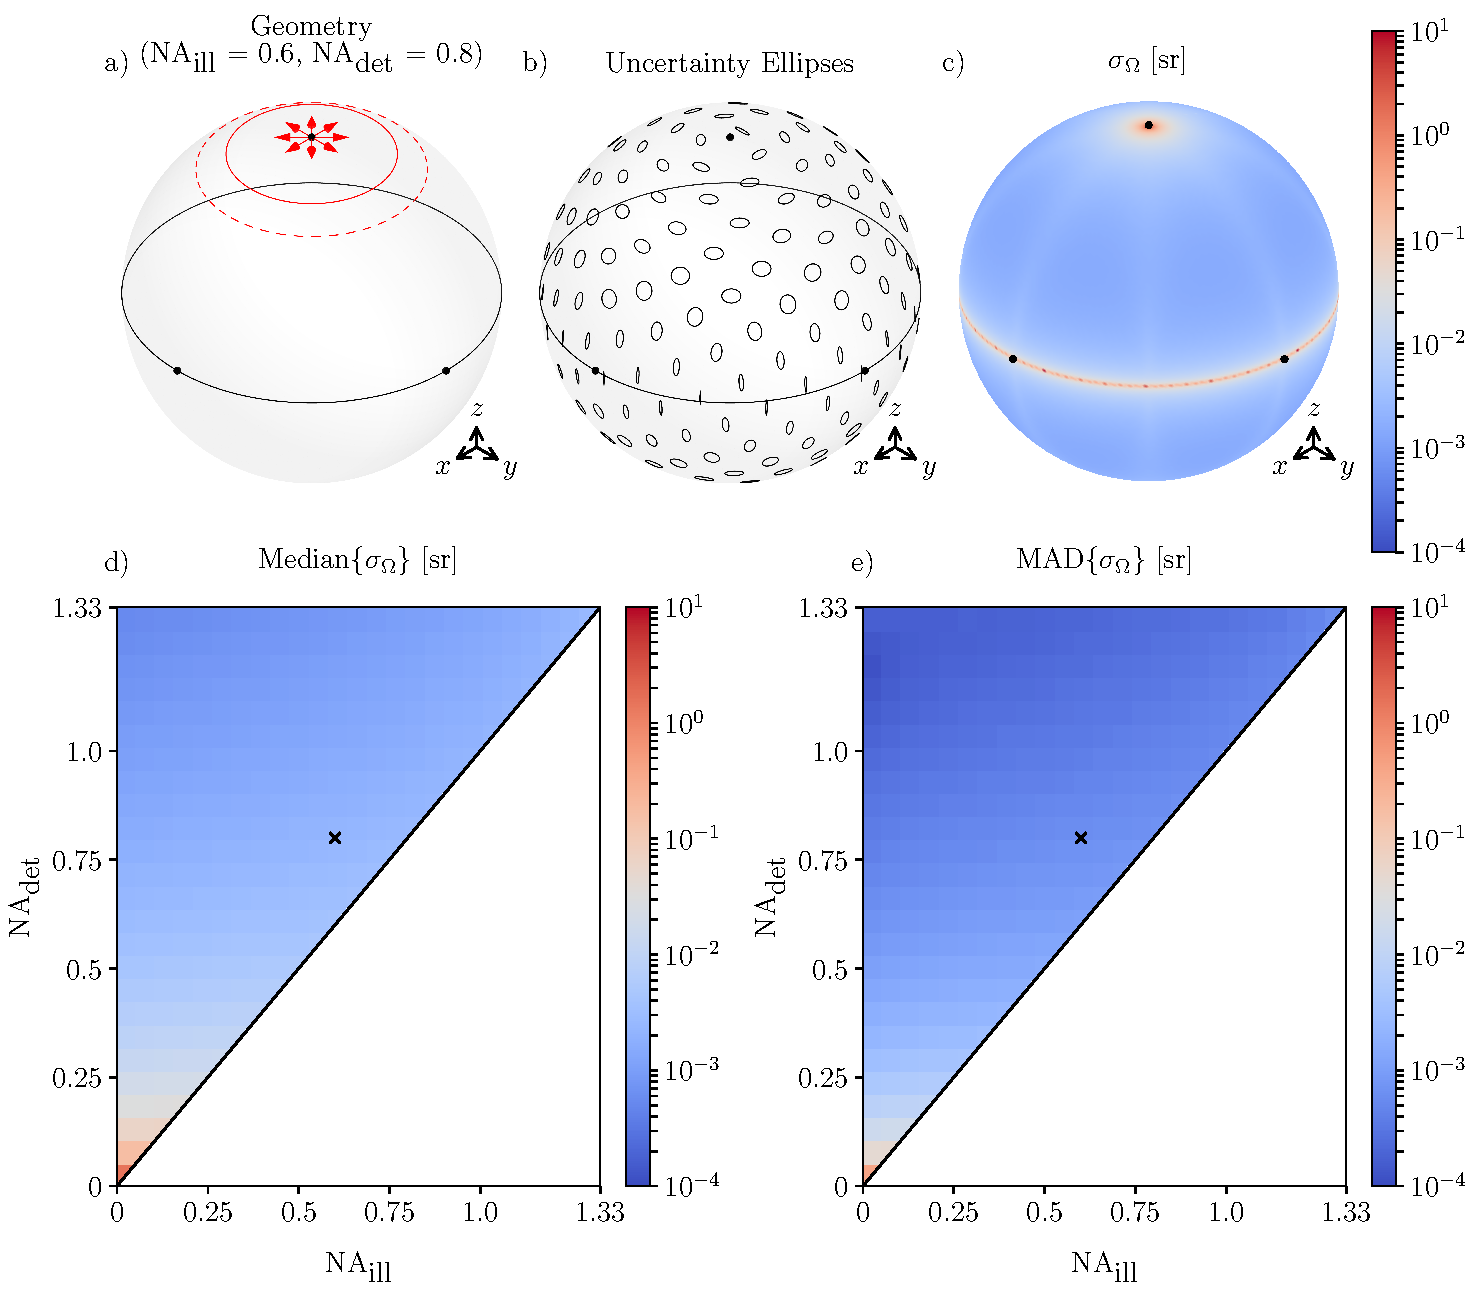
\includegraphics[width=\textwidth]{single-arm}
\caption{Single-view microscope with varying illumination and detection NA. a)
  Schematic of a single-view four-polarization epi-illumination microscope. The
  red arrows indicate the four illumination polarization orientations---one for
  each intensity measurement. b) Uncertainty ellipses for the microscope in
  a). The ellipses indicate the relative size of the uncertainty in different
  directions, not the absolute size of the uncertainty. c) Solid-angle
  uncertainty for the microscope in a). The solid-angle uncertainty is a measure
  of the absolute size of the uncertainty in all directions. d) Median of the
  solid-angle uncertainty as a function of illumination and detection NA. e) MAD
  of the solid-angle uncertainty as a function of illumination and detection
  NA. The microscope configuration in a), b), and c) is indicated by a cross in
  d) and e).}
\label{fig:single-arm}
\end{figure}

Figures \ref{fig:symmetric-widefield} and \ref{fig:double-arm} show our results
for dual-view symmetric designs. We illuminate from one objective and detect
from the other for four polarization orientations, then we repeat the
polarization orientations with the same objectives in reversed roles. In Fig.
\ref{fig:symmetric-widefield} we sweep through the NA of both objectives and the
angle between the objectives while considering steric constraints. Note how
adding a second view removes the high uncertainty region in the transverse
plane. The dual-view microscope still has high uncertainty regions near the
optical axes, but the uncertainty is reduced by almost two orders of magnitude
compared to the single-view microscope. We find that the lowest median of the
solid-angle uncertainty occurs with the largest possible NA objectives. We also
find that increasing NA always lowers the MAD, but orthogonal arms are not
always optimal. At large NA, it is advantageous to move the objectives together
or against the cover slip. Given the high uncertainty in the transverse plane
for a single-view shown in Fig. \ref{fig:single-arm}(c), we can see why oblique
views perform better than orthogonal views---oblique views are complementary
because the regions of high orientation uncertainty from each view do not
overlap.

\begin{figure}[htbp]
\centering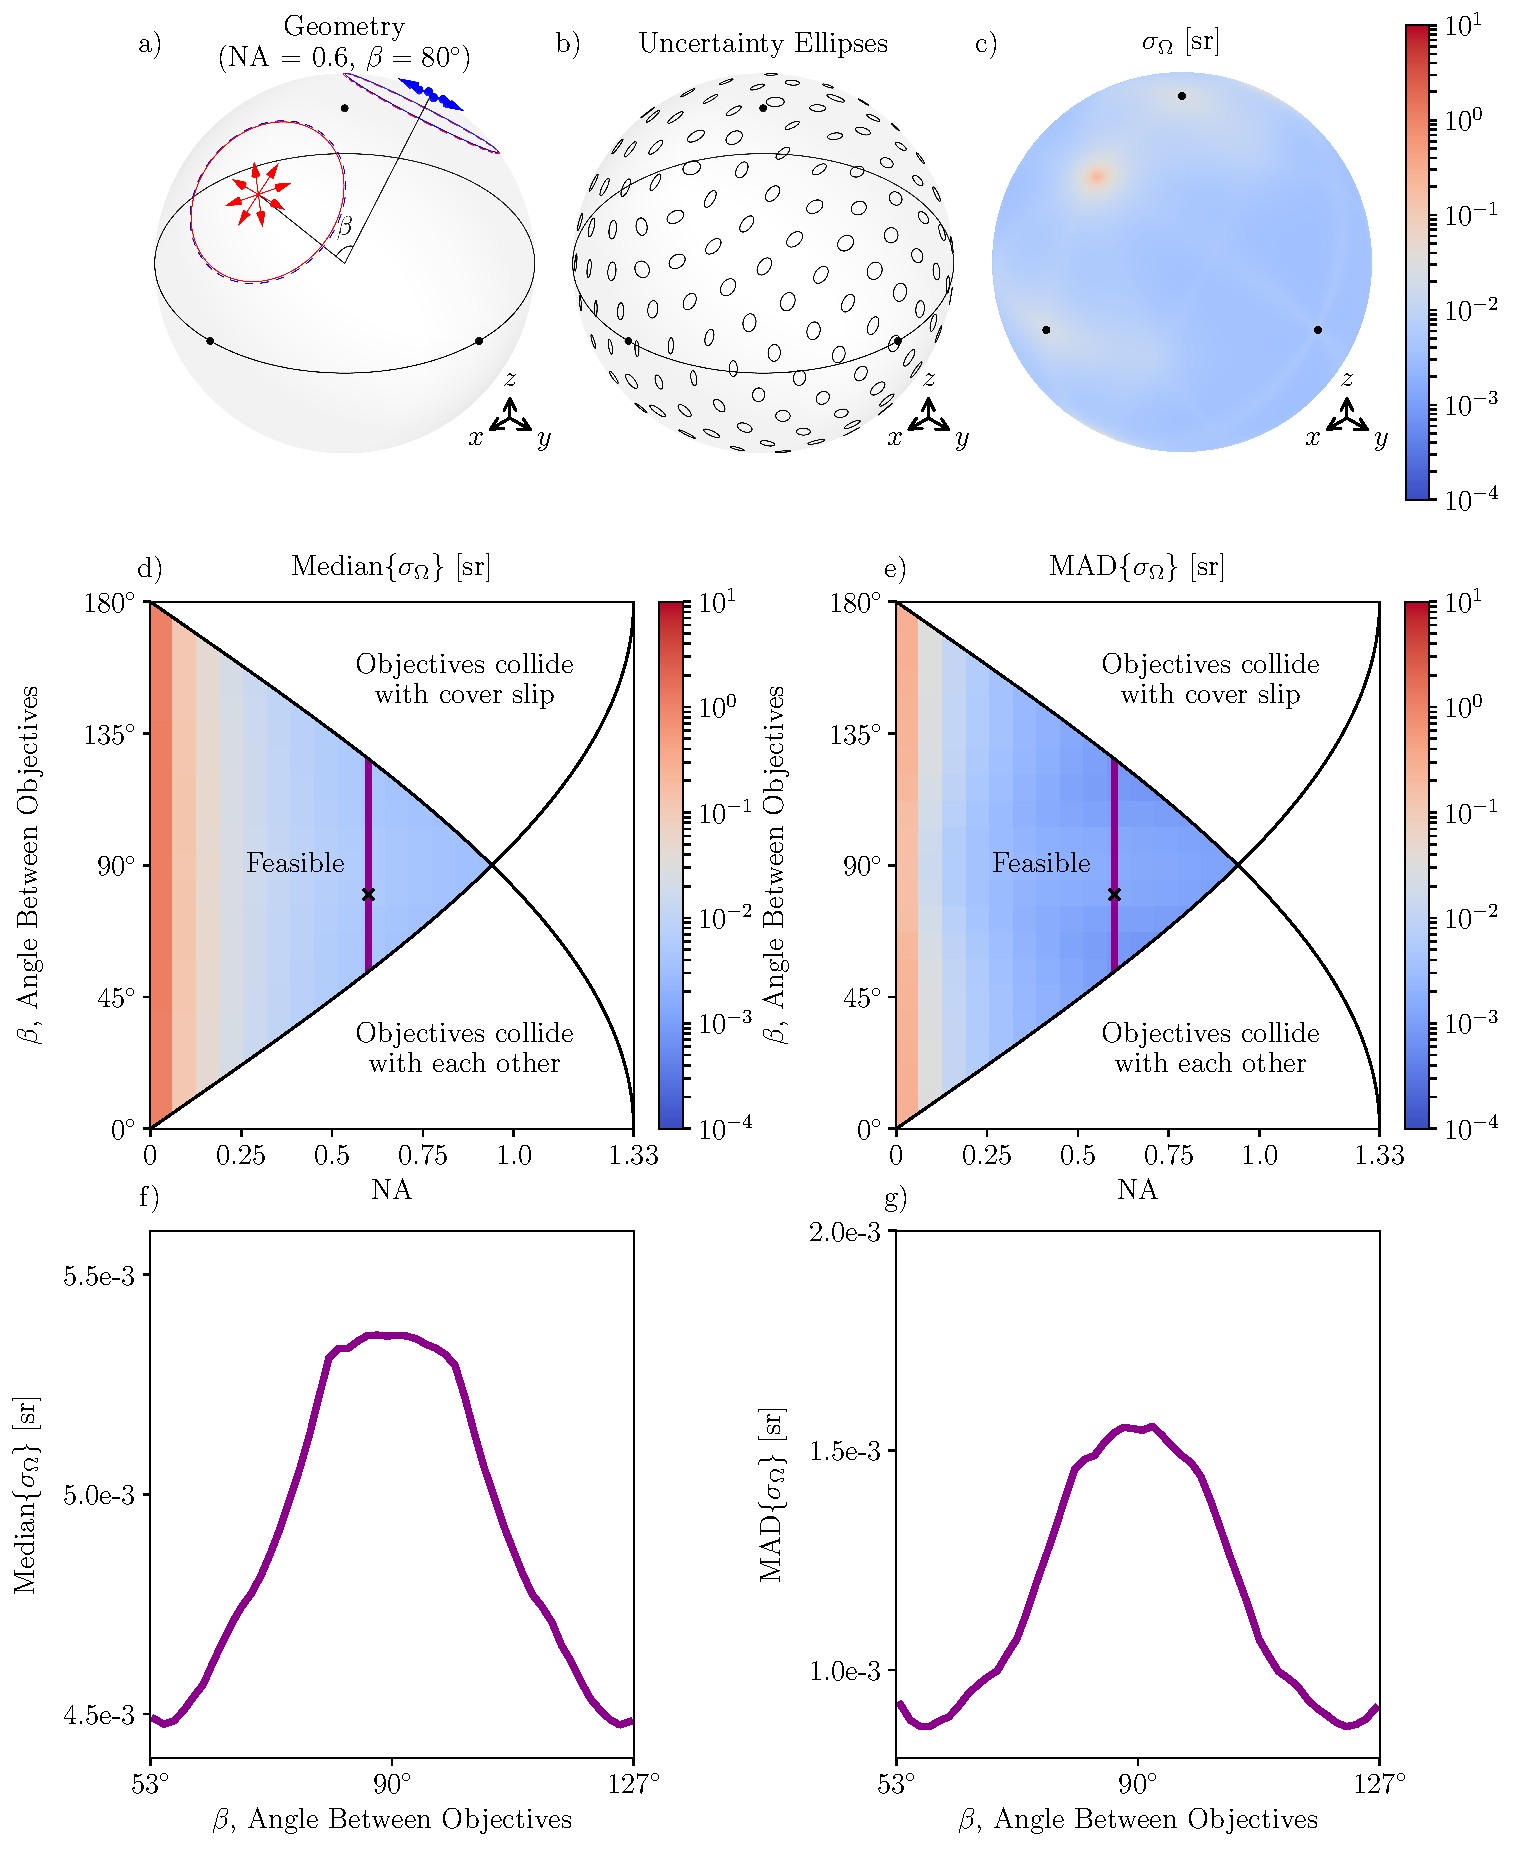
\includegraphics[width=\textwidth]{symmetric-widefield}
\caption{Dual-view symmetric designs with varying NA and angle between
  objectives. a) Schematic of the microscope. We illuminate with the first
  objective (red solid) and detect from the second objective (red dashed). Then
  we illuminate from the second objective (blue solid) and detect from the first
  objective (blue dashed). b) Uncertainty ellipses for the microscope in a). The
  ellipses indicate the relative size of the uncertainty in different
  directions, not the absolute size of the uncertainty. c) Solid-angle
  uncertainty for the microscope in a). The solid-angle uncertainty is a measure
  of the absolute size of the uncertainty in all directions. d) Median of the
  solid-angle uncertainty as a function of NA and the angle between the
  objectives. e) MAD of the solid-angle uncertainty as a function of NA and the
  angle between the objectives. The microscope configuration in a), b), and c)
  is indicated by a cross in d) and e). f) Median of the solid-angle uncertainty
  as a function of the angle between the objectives when NA=0.6. g) MAD of the
  solid-angle uncertainty as a function of the angle between the objectives when
  NA=0.6. The profile in f) and g) is taken along the purple line in d) and e).}
\label{fig:symmetric-widefield}
\end{figure}

Figure \ref{fig:double-arm} shows our results when we used a dual-view symmetric
orthogonal design and varied the illumination and detection NA. Our results are
similar to the single-view case in Fig. \ref{fig:single-arm}. We find that
optimal designs use a small illumination NA and a large detection NA. As we
discussed in Section \ref{excitation}, low-NA illumination is
approximately equivalent to light-sheet illumination for the task of estimating
the orientation of dipoles. Therefore, the preference for low-NA
illumination also implies that dual-view light-sheet illumination geometries are
an excellent choice for uniformly reconstructing the orientation of single
dipoles.

\begin{figure}[htbp]
\centering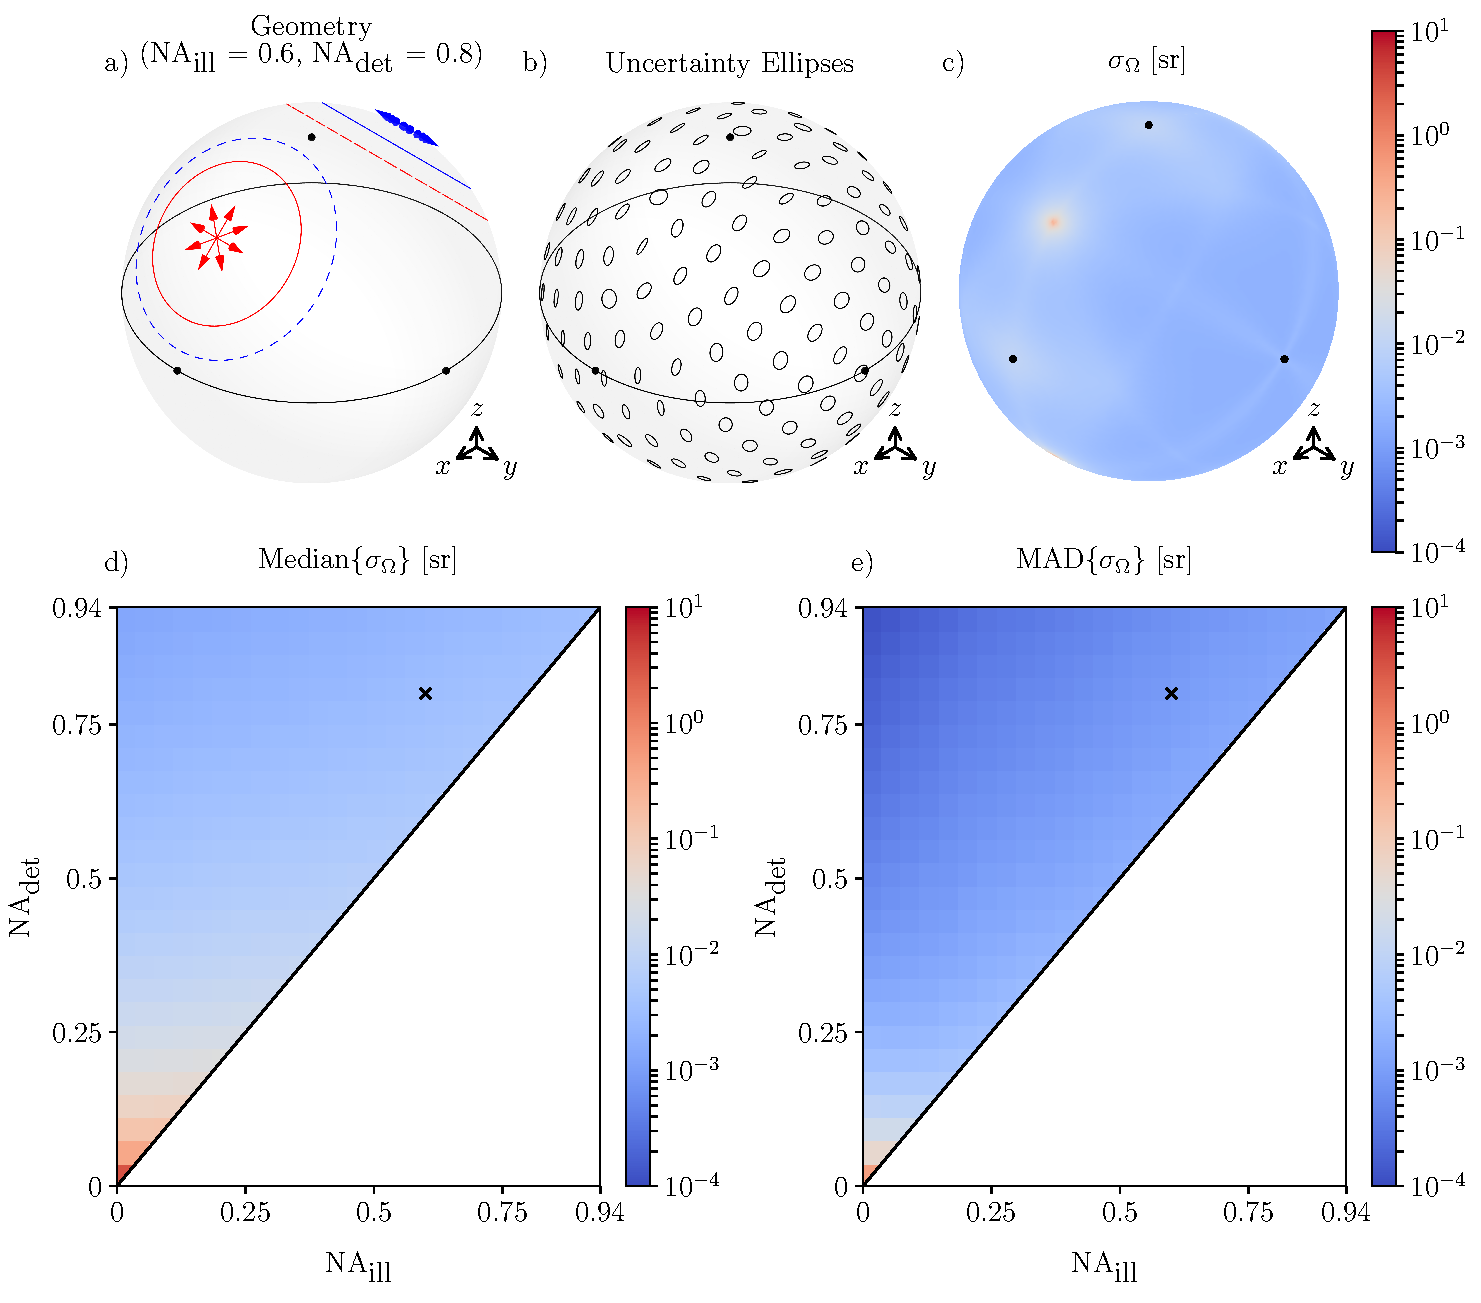
\includegraphics[width=\textwidth]{double-arm}
\caption{Dual-view symmetric orthogonal designs with varying
  illumination and detection NA. a) Schematic of the microscope. b) Uncertainty
  ellipses for the microscope in a). The ellipses indicate the relative size of
  the uncertainty in different directions, not the absolute size of the
  uncertainty. c) Solid-angle uncertainty for the microscope in a). The
  solid-angle uncertainty is a measure of the absolute size of the uncertainty
  in all directions. d) Median of the solid-angle uncertainty as a function of
  illumination and detection NA. e) MAD of the solid-angle uncertainty
  as a function of illumination and detection NA. The microscope configuration
  in a), b), and c) is indicated by a cross in d) and e).}
\label{fig:double-arm}
\end{figure}

Figure \ref{fig:asymmetric-double} shows our results for dual-view asymmetric
light-sheet illumination designs. We used light-sheet illumination on both sides
and kept the objectives orthogonal so that the light sheet from one objective
illuminates the focal plane of the other objective. Then, we swept through the
NA of one objective while maximizing the NA of the other objective so that both
objectives would touch the cover slip and each other
[$\alpha_1 + \alpha_2 = 90^{\circ}$ in Fig. \ref{fig:asymmetric-double}(a)]. We
swept through the NA asymmetry and the sample-exposure asymmetry while keeping
the sample irradiance constant, and found that symmetric designs are at a local
minimum of the median and MAD of the solid-angle uncertainty. We also found that
at extreme asymmetries where the exposure from the low-NA arm is much larger
than the exposure from the high-NA arm [top-left and bottom-right corners of
Figs. \ref{fig:asymmetric-double}(d) and 6(e)] the median and MAD are comparable
to the symmetric light-sheet microscope. This means that if a very high-NA
objective is available and a low-NA objective can provide light sheet
illumination, this microscope will perform comparably with a dual-view
microscope with two medium-NA objectives. Note that this asymmetric exposure
configuration maximizes the use of the high-NA detection objective---if a
high-NA objective is available it should be used for detection as much as
possible. Figure \ref{fig:asymmetric-double} also shows that designs with
slightly asymmetric NA can trade off a low solid-angle uncertainty median for a
low solid-angle uncertainty MAD by changing the sample exposure ratio.

\begin{figure}[htbp]
  \centering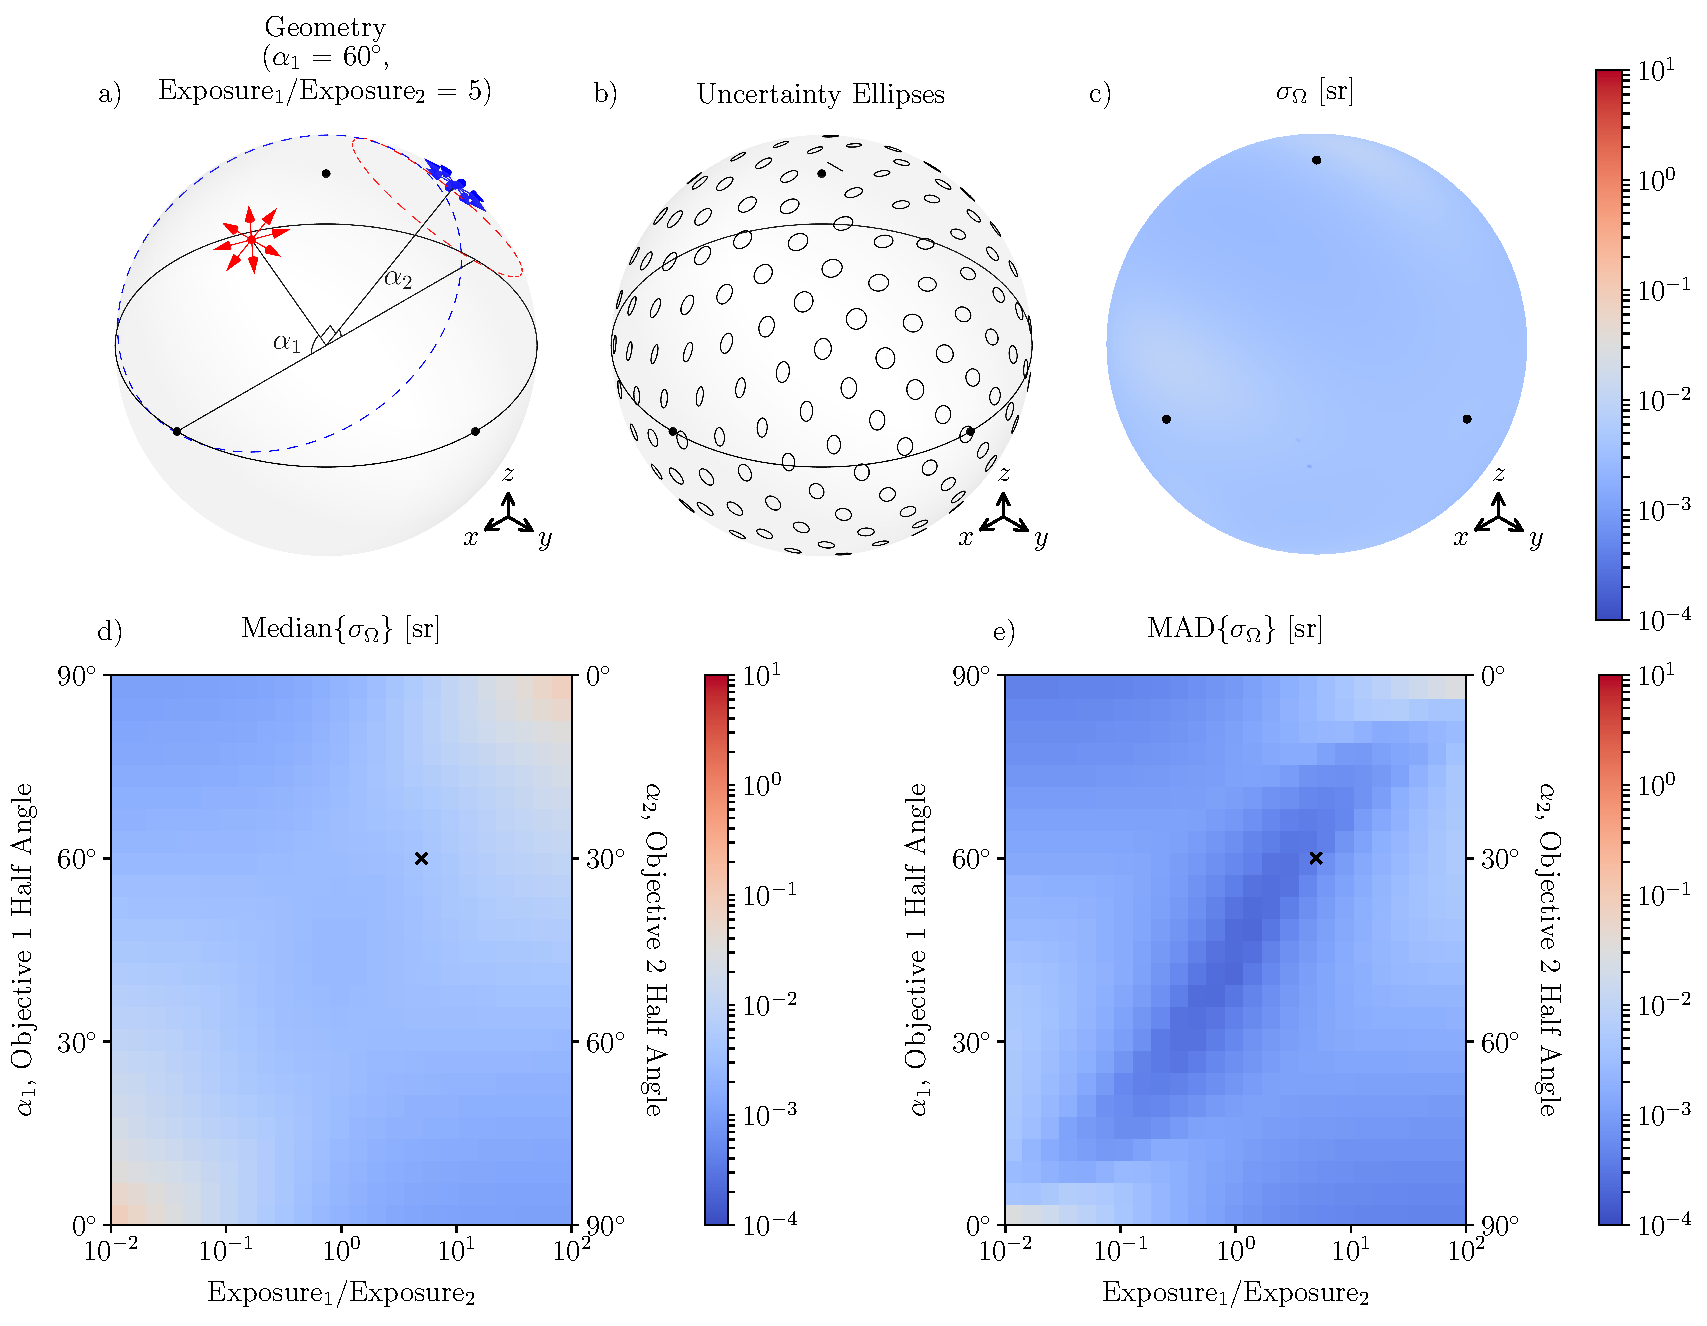
\includegraphics[width=\textwidth]{asymmetric-double}
  \caption{Dual-view asymmetric light-sheet illumination designs with varying NA
    and sample exposure asymmetry. a) Schematic of the microscope. b)
    Uncertainty ellipses for the microscope in a). The ellipses indicate the
    relative size of the uncertainty in different directions, not the absolute
    size of the uncertainty. c) Solid-angle uncertainty for the microscope in
    a). The solid-angle uncertainty is a measure of the absolute size of the
    uncertainty in all directions. d) Median of the solid-angle uncertainty as a
    function of NA and sample exposure asymmetry. e) MAD of the solid-angle
    uncertainty as a function of NA and sample exposure asymmetry. The
    microscope configuration in a), b), and c) is indicated by a cross in d) and e).}
\label{fig:asymmetric-double}
\end{figure}

Table 1 shows a summary of our evaluation metrics for microscopes in each
class. The single-view microscope with a small illumination NA and high
detection NA has the lowest solid-angle uncertainty median but the largest max
and fourfold degeneracy. The dual-view oblique symmetric microscope with an
intermediate NA performs reasonably well on all three metrics, while the
dual-view orthogonal symmetric light-sheet microscopes with large NA perform
very well on all three metrics.

% \begin{table}[ht!]
% \centering
% \caption{Comparison of designs in each class of microscope. All solid-angle
%   uncertainty statistics are in steradians.}
% \begin{tabular}{lllll}
%   \toprule

%   Microscope Type&$n$-fold&Max\{$\sigma_{\Omega}$\}&Median\{$\sigma_{\Omega}$\}&MAD\{$\sigma_{\Omega}$\}\\ 
%     &Degeneracy&&&\\\midrule
% Single-view (NA${}_\textrm{ill}$=0, NA${}_\textrm{det}$=1.1)&4&3.04$\times 10^{0}$&8.20$\times 10^{-4}$&1.48$\times 10^{-4}$ \\ 
%   Dual-view oblique symmetric (NA=0.6, $\beta$=53${}^{\circ}$)&2&1.35$\times 10^{-1}$&4.49$\times 10^{-3}$&9.17$\times 10^{-4}$\\
% Dual-view orthogonal symmetric light-sheet (NA=0.8)&2&6.23$\times 10^{-3}$&1.79$\times 10^{-3}$&1.65$\times 10^{-4}$\\  
% Dual-view orthogonal symmetric light-sheet (NA=0.94)&2&3.13$\times 10^{-3}$&1.28$\times 10^{-3}$&1.14$\times 10^{-4}$\\
% \bottomrule
% \end{tabular}
% \end{table}

\begin{table}[ht!]
\centering
\caption{Comparison of designs in each class of microscope. All solid-angle
  uncertainty statistics are in steradians.}
\begin{tabular}{lllll}
  \toprule
  Microscope Type&Single-view&Dual-view&Dual-view&Dual-view\\ 
    &NA${}_\textrm{ill}$=0&oblique&orthogonal&orthogonal \\
    &NA${}_\textrm{det}$=1.1&symmetric&symmetric&symmetric\\
    &&NA=0.6&light-sheet&light-sheet\\  
    &&$\beta$=53${}^{\circ}$&NA=0.8&NA=0.94\\\midrule
  
  $n$-fold Degeneracy&4&2&2&2\\
  Max\{$\sigma_{\Omega}$\}&3.04$\times 10^{0}$&1.35$\times 10^{-1}$&$6.23\times 10^{-3}$&3.13$\times 10^{-3}$\\
  Median\{$\sigma_{\Omega}$\}&8.20$\times 10^{-4}$&4.49$\times 10^{-3}$&$1.79\times 10^{-3}$&1.28$\times 10^{-3}$\\
  MAD\{$\sigma_{\Omega}$\}&1.48$\times 10^{-4}$&9.17$\times 10^{-4}$&$1.65\times 10^{-4}$&1.14$\times 10^{-4}$\\
\bottomrule
\end{tabular}
\end{table}


\section{Discussion and conclusions}\label{discussion}
In this work we have developed a model to predict the intensities measured by
polarized illumination microscopes in a wide range of geometries, developed
metrics to measure the ability of a microscope design to estimate the
orientation of single dipoles, and used these metrics to compare a wide
range of microscope designs. Our main result is a short list of design
heuristics that can be used to design polarized-illumination single-dipole
orientation microscopes:
\begin{itemize}
\item Single-view microscopes benefit from a small illumination NA and a large
  detection NA with $\alpha \approx 65^{\circ}$.
\item Dual-view microscopes outperform single-view microscopes along several
  metrics. Dual-view microscopes have fewer degeneracies, lower median and MAD
  solid-angle uncertainty, and no high solid-angle uncertainty region in the
  transverse plane.
\item High-NA dual-view microscopes are optimal when the two views are
  oblique. Oblique views are complementary because their high uncertainty
  transverse planes do not overlap.
\item Symmetric NA dual-view orthogonal light-sheet microscopes provide a good
  compromise between cost, solid-angle uncertainty median, and solid-angle
  uncertainty MAD. Asymmetric NA dual-view orthogonal light-sheet microscopes
  can improve the solid-angle uncertainty median or MAD by changing the sample
  exposure ratio between the two views.
\end{itemize}

Our results are limited in several ways. First, we only consider single
molecules in homogeneous environments whose absorption and emission dipoles are
parallel. We ignore light reflected from the cover slip and any other
inhomogeneities in the sample. If we considered light reflected from the cover
slip we expect that the results would put a lower weighting on large detection
NAs because we would collect more light. Second, we only considered ideal,
aplanatic, polarization-preserving objectives. In practice, these conditions are
not always satisfied. For example, the power from high-NA rays is usually
apodized by a factor of $\frac{n}{\cos\Theta}$ \cite{nov2006}. Therefore, our
results are most accurate for paraxial rays and get progressively worse for
non-paraxial rays, although our major conclusions would not change if we
included this apodization factor. The main advantage of ignoring apodization is
the tractability of the problem---we have provided approximate closed-form
solutions for the illumination and detection efficiencies that have allowed us
to draw useful design conclusions. Third, we have used a Poisson noise model
which ignores noise introduced by the detector. Detector noise can be a large
fraction of the total noise at low intensities, so including detector noise
would increase the informational value of high intensity
measurements. Therefore, we expect that including the effects of detector noise
would favor microscopes with a large detection NA. Finally, we have focused on
the task of estimating the orientation of dipoles and ignored the equally
important task of estimating their location. The task of jointly estimating the
orientation and location of single dipoles from multiple views is a topic for
future work.

To compare the microscopes in this paper we used a fixed irradiance incident on
the sample. We think that this is the fairest way to compare microscopes with
different numbers of intensity measurements. However, in cases where sample
irradiance and time are not an issue it may be more useful to compare
microscopes with the same total detection irradiance per measurement. This
comparison would favor microscopes with many intensity measurements even more
that the results in this paper because equal detection irradiance would improve
photon counting statistics.

% \hypertarget{temporal}{{\color{urlblue} We also chose to compare microscopes
%     with a fixed irradiance incident on the sample so that all of the
%     microscopes had the same temporal resolution. Given a fixed irradiance, the
%     main factor that limits the temporal resolution of an orientation microscope
%     is the brightness of the fluorophore (the rate of photon emission from the
%     fluorophore). The orientation of bright fluorophores can be determined more
%     quickly than dim fluorophores at the same level of accuracy because bright
%     fluorophores generate measurements with a higher signal-to-noise ratio.}}

We have considered single- and dual-view microscopes in a variety of cases, but
other multiview microscopes can be analyzed with the framework we have
developed. Wu et. al. have developed a three-view design with a third objective
below the cover slip\cite{wu2016}. Light-field detection schemes are also a type
of multiview microscope\cite{levoy2006}, and we plan to extend our analysis to
this case in future work.

The models in this paper only consider estimating the orientation of fixed
dipoles, but real dipoles change their orientation during
measurement. Therefore, it is necessary to comment on the applicability of our
results to dynamic dipoles. In general, using the models in this paper to
estimate the orientation of rotating dipoles will lead to incorrect
results. However, if a dipole rotates through a small solid angle during the
measurement, the models in this paper will give a slightly biased estimate of
the average orientation of the dipole. The direction and size of the bias has
not been characterized in detail. In future work we will model dynamic dipoles
and attempt to estimate the average dipole orientation and the dipole's
orientation distribution. Single-view polarized illumination techniques have
already been used to study the orientation distribution of ensembles of dynamic
dipoles \cite{mehta2016, backer2016}, but multiview polarized illumination
microscopes have not been investigated for this purpose.

We have only considered polarized illumination. In the introduction
we discussed why we prefer polarized illumination to polarized detection, but
there is information to be gained by adding polarized detection to the
techniques discussed in this paper. Adding a polarization splitter to the
detection arm can increase the information available for reconstructing the
orientation of a single dipole without increasing the acquisition time.

We conclude that multiview microscopes are useful tools for determining the
orientation of single dipoles. Using simple design heuristics, we can design
polarized illumination multiview microscopes that can determine the orientation
of single dipoles with a small and uniform orientation uncertainty.

\section*{Funding}
National Institute of Health (NIH) (R01GM114274, R01EB017293).

\section*{Acknowledgments}
TC was supported by a University of Chicago Biological Sciences Division
Graduate Fellowship. HS and PL were supported by Marine Biological Laboratory
Whitman Center Fellowships. HS was supported by the Intramural Research
Programs of the National Institute of Biomedical Imaging and Bioengineering.

\section*{Disclosures}
The authors declare that there are no conflicts of interest related to this article.

\end{document}
